
\section{Motivation} \label{sec:motivation}
Data center energy efficiency has become of crucial importance in recent years due to its high economic, environmental, and performance impact. For example, the leading petaflop supercomputers consume a range of 1–18 MW of electrical power, with 1.5 MW on average, which can be easily translated into millions of dollars per year in electricity bills \cite{Group2012HandbookSahni}.
Data center energy consumption was estimated to be between 1.1\% and 1.5\% of worldwide electricity usage in 2010 \cite{Dayarathna2016DataSurvey,Corcoran2017EmergingICT}, generating as much pollution as a nation such as Argentina  \cite{Mathew2012Energy-awareNetworks}.
In some cases, the power costs exceed the cost of purchasing hardware~\cite{Rivoire2007ModelsOptimizations}.
Furthermore, the energy costs of powering a typical data center doubles every five years~\cite{Buyya2013Introduction}.
Therefore, with such a steep increase in power use, electricity bills have become a significant expense for today's data centers \cite{Poess2008EnergyCenters,Gao2013QualityCenters}. 
For these reasons, data center energy efficiency is now considered a primary concern for data center operators, often ahead of the traditional considerations of availability and security.

There are several approaches for green computing, from electrical materials to circuit design, systems integration, and software. These techniques may differ, but they share the same goal---to substantially reduce overall system energy consumption without a corresponding negative impact on delivered performance.
The processor and main memory are  the components that usually dominate power consumption, as shown in \cref{fig:powerbreakdown}.
The processor can consume as much as 50\% of the total energy~\cite{Fan2007PowerComputer, Barroso2007TheComputing, Malladi2012TowardsDRAM}. For that reason, modern processors incorporate several features for power management~\cite{Rotem2012Power-managementBridge, Brown2005ACPILinux, Hackenberg2015AnProcessor, Intel20200thLake}, such as dynamic power management (DPM) and dynamic voltage and frequency scaling (DVFS). 
DPM encompasses a set of techniques for obtaining energy-efficient computing by deactivating or reducing the system components' performance when they are idle or partially utilized~\mbox{\cite{Shuja2012Energy-efficientCenters, Benini2000AManagement}}.
DVFS allows the frequency and voltage to be adjusted in run-time depending on current needs.


\begin{figure}[H]
	\centering
	\captionsetup[subfigure]{justification=centering}
	
	\begin{subfigure}[b]{0.45\textwidth}
		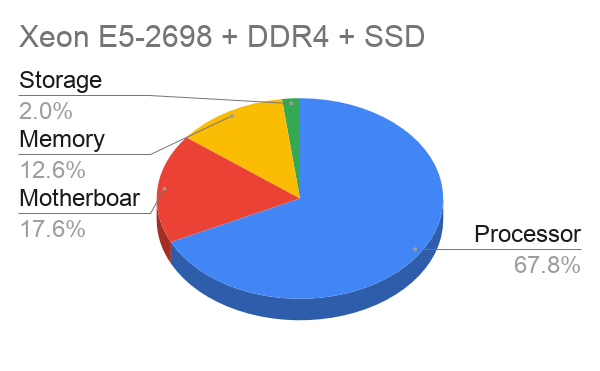
\includegraphics[width=\textwidth]{models/figures/power_breakdown/Xeon E5-2698 + DDR4 + SSD.png}
		\caption{}
		\label{fig:powerbreakdown_a}
	\end{subfigure}
	%
	\begin{subfigure}[b]{0.45\textwidth}
		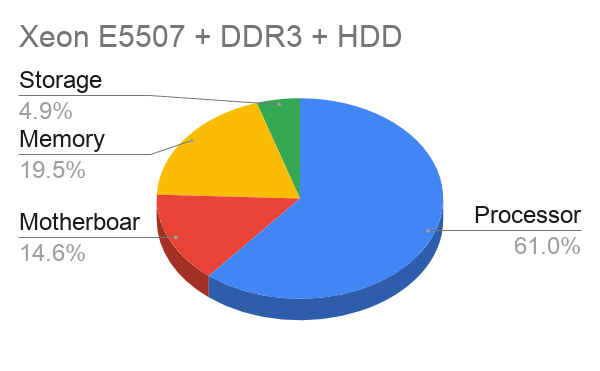
\includegraphics[width=\textwidth]{models/figures/power_breakdown/Xeon E5507 + DDR3 + HDD.png}
		\caption{}
		\label{fig:powerbreakdown_b}
	\end{subfigure}
	
	\hfill
	\caption{Power breakdown of a typical node of an HPC cluster at full use. The system used in this study (\textbf{a}) was built in 2016 and equipped with two Intel Xeon E5-2698, 128 GB of DDR4 memory and SSD as storage, while (\textbf{b}) the case study in \cite{Malladi2012TowardsDRAM} was built in 2012 and equipped with two Xeon E5507, 32GB of DDR3 memory and HDD as storage.}
	\label{fig:powerbreakdown}
\end{figure}

DVFS is motivated by the well-known fact that frequency and power have a near-cubic relationship \cite{Dayarathna2016DataSurvey, Group2012HandbookSahni}; this implies that running the CPU at a lower frequency causes a linear reduction in performance and a near-cubic reduction in power, which could lead to a near-square reduction in CPU energy.
Because of this, it is possible to achieve dramatic energy savings just with frequency control, depending on the system and its architecture.
Although very promising, the system software has yet to determine when and what voltage and frequency to use when running applications.
Otherwise, not only will performance deteriorate, but, in the worst case, energy consumption would also increase  \cite{Group2012HandbookSahni}.
Indeed, reducing the frequency results in a longer execution time, which increases the energy consumption of other system components, such as memory and disks.
There is also an overhead of time and energy associated with a voltage and frequency switch that needs to be considered.
Thus, finding the most appropriate voltage and frequency to use in all circumstances is not easy.
Therefore, since its introduction in 1994 \cite{Group2012HandbookSahni}, there has been a tremendous amount of research on DVFS algorithms.

The DPM technique can achieve substantial energy savings on systems where the static power is high, or the system remains inactive for a long time.
In that case, the problem is to determine when and which components to turn on/off.
With DPM, energy savings of 70\% have been reported~\cite{Shuja2012Energy-efficientCenters, Benini2000AManagement}. 

However, at the same time, while these power-saving techniques reduce system energy, they can compromise  performance leading  to a complex trade-off that needs to be carefully exploited to produce more energy-efficient algorithms.
Indeed, this study investigates whether the construction of an energy consumption model of an application can lead to significant energy savings.

We propose an analytical energy model for a given application in the function of the two control variables present in most HPC systems: CPU operating frequency and number of active cores. The model is composed of three application-dependent parameters and three parameters relating to the architecture of the system. The application parameters incorporate characteristics of the percentage of parallelism and the input size. The system architecture parameters include power-related and technology-dependent components, such as dynamic, static, and leakage power.

\section{Objectives} \label{sec:objectives}


\section{Contributions*} \label{sec:contributions}

Although much work has been done on DVFS, the focus is still on the consumer electronics and laptop markets. 
For HPC, the notion of energy perception is relatively new~\cite{Feng2003MakingSupercomputing}. 
Moreover, the operational characteristics of non-HPC and HPC systems are significantly different. 
First, the workload on non-HPC systems is very interactive with the end-user, but the workload on the HPC platform is not.
Second, activities conducted on a non-HPC platform tend to share more machine resources.
In contrast, in HPC, each job often runs with dedicated resources. 
Third, an HPC system is usually much larger than a non-HPC system, making it more challenging to gather information, organize, and execute global decisions.
Therefore, it is worthwhile to investigate whether a DVFS scheduling algorithm, which works well for conventional computing, remains effective for HPC.

Our paper proposes a full-system energy model based on the CPU frequency and the number of cores. The model aims to understand and optimize the energy behavior of parallel applications in HPC systems according to application parameters, such as the degree of parallelism and CPU parameters related to dynamic and static power. The proposed model differs from existing ones, including the frequency and number of cores in the same equation for estimating the energy for a specific application in a given configuration. This model can serve as a base for considering DVFS and DPM optimization problems, including frequency and active cores. It can also be used to analyze the contribution of each parameter (ex: level of parallelism) to energy consumption. Furthermore, the number of cores is essential in HPC since applications are designed to run on multiple cores.

The proposed energy model is the product of an application-agnostic power model and an architecture-specific application performance model. The power model is based on the CMOS logic gates power draw as a function of the frequency~\cite{Sarwar1997CmosCalculation, Butzen2007LeakageGates} augmented to include the number of cores. The performance model is based on Amdahl's law \cite{Amdahl1967ValidityCapabilities, Eyerman2010ModelingDesign, Gustafson1988ReevaluatingLaw}, which can be used to estimate runtime in multi-core systems. In addition, this model has been extended to include execution frequency and input size, characterizing the application on the target architecture.


\cref{tab:related_work} summarizes the models comparing the system dependencies and the controllable variables.
\begin{table}[H]
	\footnotesize
	\caption{Related work summary.\label{tab1}}
	\setlength{\tabcolsep}{2.3mm}\begin{tabular}{cccc}
		\toprule
		%\begin{adjustwidth}{-\extralength}{0 cm}
		
		\textbf{Model}  & \textbf{System Dependency}       & \textbf{Variable}                     & \textbf{Controllable Variables}         \\ \midrule
		Merkel et al. \cite{Merkel2006BalancingSystems} & performance counters    & number of activities & - \\
		Roy et al. \cite{Roy2013AnAlgorithms}&performance counters &io operations, total time    & - \\
		Yakun et al. \cite{Shao2013EnergyProcessor}&number of instructions &frequency&frequency \\
		Lewis et al. \cite{Lewis2008Run-timeSystems}&energy of subcomponents&energy of subcomponents & - \\
		Mills et al. \cite{Mills2014EnergySystems}&power of subcomponents&total time, frequency & frequency \\ 
		Our model & - & frequency, cores, input size & frequency, cores, input size\\ \bottomrule
	\end{tabular}
	%\caption{Related work summary}
	\label{tab:related_work}
	%\bottomrule
\end{table}

The main contributions of the proposed model are:


% Contribuições por capitulo...
\begin{itemize}
	\item Simple model: faster to fit and compute, good for DVFS and DPM optimization.
	\item Parameters with logical meaning: helps to understand the contribution of each specific term.
	\item Analytical analysis: several analyses can be derived from the equation.
	\item Controllable variables: the equation is in the function of parameters that we can control directly.
\end{itemize}

\section{Organization}